\newcommand{\lsql}[1]{\lstinline[language=SQL,prebreak=]!#1!}

\lab{SQL and Relational Databases}{SQL}
\objective{Understand concepts of a relational database and the fundamentals of the SQL language via SQLite.}
\label{lab:sql_rdb}

When working with large amounts of data, it is important to be able to quickly find and retrieve interesting information.
Fortunately, there is a way to handle such massive amounts of data in a reasonably efficient way: a database.
A database is simply a structured repository of data, and it allows us to store and retrieve information very quickly.
It is managed by a \emph{database management system}, or DBMS.
The DBMS is software that allows users to interact directly with the database.

\section*{Relational Databases}
A \emph{relational database} is paradigm for organizing data inside of a database.
In this paradigm, the data are broken down into tuples of information.
These tuples are then grouped into tables, or \emph{relations}, each of which is simply a set of tuples.
Each table has a \emph{schema} that defines the attributes of the tuples within the table.
If we fix an order to the attributes in the schema, we can think of each attribute as a column
of the table, and each tuple as a row of the table. See Figure \ref{fig:relation} for an illustration of
these ideas.

As an example, suppose we have demographic data for a large number of individuals.
If we are interested in the gender and age of the individuals, we might make a table
with schema (Name, Gender, Age). This table would consist of several 3-tuples, such as
(Jane Doe, F, 20). Alternatively, we can view this table as having three columns
and as many rows as there are individuals within our data set.
We might also create a table with schema (Name, Employment Status, Income, Education).

In the relational paradigm, there must be at least one attribute in each schema that can act as a \emph{primary key}.
This can uniquely identify each tuple of the table.
It is common to use an ID number or other such unique information for the primary key.
In our example above, the ``Name" attribute acted as a primary key. However, this attribute only works as a primary
key provided no two individuals within the data set have the same name.
\begin{figure}
\centering
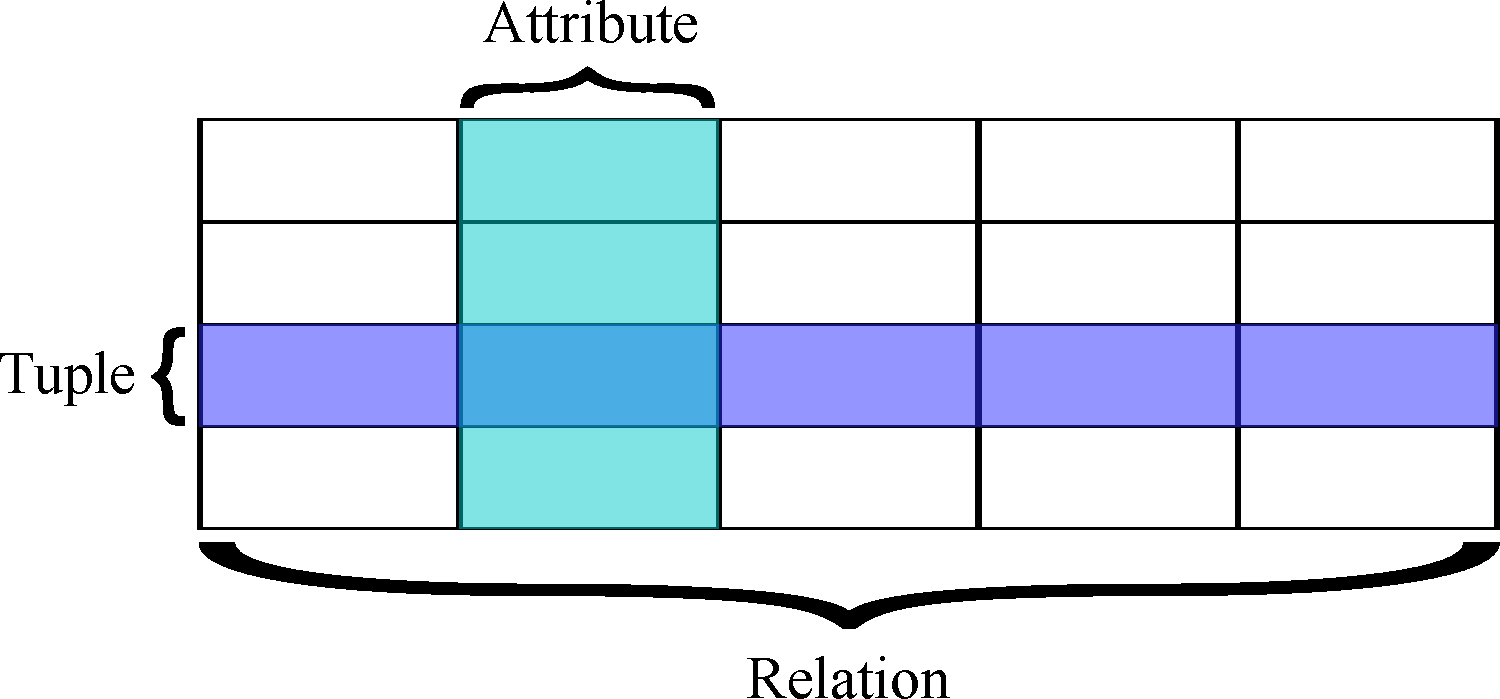
\includegraphics[width=\textwidth]{rdb_table.pdf}
\caption{Elements of a relation.}
\label{fig:relation}
\end{figure}

One important feature of a database is the \emph{transaction}, which is a conceptual protocol for
interacting with the database.
Most relational databases are transactional databases.
The best way to conceptualize this is imagine that your database is like a bank.
Your connection the database is analogous to the bank teller.
When you make one or more deposits and withdrawals, you are making a transaction.
A database transaction should have certain properties to protect the integrity of the data.
These properties are succinctly captured in the acronym of ACID, and
compliance with these properties is an important feature of transactional databases.
Let us consider the four ACID properties: atomic, consistent, isolation, and durable.
\begin{description}
\item[Atomic.] Each transaction should be all or nothing.  If some error occurs in the middle of a transaction,
no changes are made to the database.  Changes are only made during error-free transactions.  This is especially
useful if a transaction is interrupted due to power failure, or some other type of unforeseen error.
\item[Consistent.] Ensure that the database is always left in a valid state.  This ensures that any transaction
satisfies all rules and constraints of the database.
\item[Isolation.] The final effect of concurrent transactions is equivalent to the final effect of each transaction
in serial.  This essentially means that if multiple users perform several transactions in parallel, none of the transactions
can depend on each other.
\item[Durable.] Once a transaction is committed, the changes are permanent regardless of any errors that may happen later.
\end{description}

\section*{Introduction to SQL}
Most common DBMSs use a variant of the SQL language to interact with the database.
SQL is an acronym for \emph{Structured Query Language}, and may be pronounced like the word ``sequel" or by saying
the letters ``s", ``q", and ``l" separately.
While SQL is not generally portable across different DBMSs, we will focus on the parts of SQL that are relatively common.
In particular, we will base our discussion on the SQLite database management system, a very popular DBMS.

SQL consists of blocks of code called statements.
Each statement is made up of clauses which may or may not require predicates.
Predicates specify conditions that can limit the effect of a clause.

\begin{info}
SQL commands are often written in all caps to help distinguish them from the other parts of the query.
It is only a matter of style.
SQLite, along with most other database managers, is case insensitive.
\end{info}

Let's look at an example SQL statement:
\begin{lstlisting}[language=SQL]
SELECT * FROM table WHERE id=3+1 AND name='Bob';
\end{lstlisting}
This statement includes a SELECT clause and a WHERE clause.
The WHERE clause contains two predicates: \texttt{id=3+1} and \texttt{name='Bob'}
These two predicates limit the effect of the SELECT clause because any resulting tuples in the table must satisfy both conditions.
This entire statement is classified as a query since it does not modify the database in any way.

SQL has several classes of statements.
The two main classes we will cover in this lab are schema (Table \ref{table:sql-schema}) and data manipulation (Table \ref{table:sql-data_manip}).
We will give you a simplified description of each command and its syntax.
You are encouraged to look up the full syntax outside of this lab.

\begin{table}
\begin{tabular}{|l|l|}
\hline
Keyword & Syntax \\
\hline
\lsql{CREATE TABLE} & \lsql{CREATE TABLE <table> (<col1> <type>, <col2> <type>, ...);} \\
\lsql{DROP TABLE} & \lsql{DROP TABLE <table>;} \\
\lsql{CREATE INDEX} & \lsql{CREATE INDEX <name> ON <table> (<col>);} \\
\lsql{DROP INDEX} & \lsql{DROP INDEX <name>;} \\
\hline
\end{tabular}
\caption{The SQL Schema commands}
\label{table:sql-schema}
\end{table}

\begin{table}
\begin{tabular}{|l|l|}
\hline
Keyword & Syntax \\
\hline
\lsql{INSERT INTO} & \lsql{INSERT INTO <table> <attributes> VALUES (<value1>, <value2>, ...);} \\
\lsql{UPDATE} & \lsql{UPDATE <table> SET (<col1>=<val1>, <col2>=<val2>, ...) WHERE <condition>;} \\
\lsql{DELETE} & \lsql{DELETE FROM <table> WHERE <condition>;} \\
\lsql{SELECT} & \lsql{SELECT <attributes> FROM <table> WHERE <condition>;} \\
\hline
\end{tabular}
\caption{The SQL Data Manipulation commands}
\label{table:sql-data_manip}
\end{table}

\section*{SQL in Python}
Python has built-in support for SQLite databases using the standard library.
Let's open a database called \texttt{test1}.
\begin{lstlisting}
import sqlite3 as sql
db = sql.connect("test1")
\end{lstlisting}
The \li{connect()} function is used to connect to a database.
If it does not already exist, then a new database will be created using string passed as the argument.
The new database was created as a file in the current working directory.
If we wanted an in-memory database, we would call \li{sql.connect('':memory:'')}.

To execute SQL commands, we need to get a cursor object from the database.
\begin{lstlisting}
cur = db.cursor()
\end{lstlisting}
The cursor object has several useful methods (Table \ref{table:cursormethods}).
\begin{table}
\begin{tabular}{|l|l|}
\hline
Method & Description \\
\hline
\li{execute} & Execute a single SQL statement \\
\li{executemany} & Execute a single SQL statement over a sequence \\
\li{executescript} & Execute a SQL script (multiple SQL commands) \\
\li{close} & Closes the cursor object \\
\hline
\end{tabular}
\caption{Cursor object methods}
\label{table:cursormethods}
\end{table}

Before creating a table, we need to  understand how SQLite stores information in a database.
SQLite uses five native data types (a simplified system from other SQL database managers).
Table \ref{table:typemap}, gives a mapping between Python and SQLite native types.
\begin{table}
\begin{tabular}{|l|l|}
\hline
Python Type & SQLite Type \\
\hline
\li{None} & \lsql{NULL} \\
\li{int} & \lsql{INTEGER} \\
\li{long} & \lsql{INTEGER} \\
\li{float} & \lsql{REAL} \\
\li{str} & \lsql{TEXT} \\
\li{buffer} & \lsql{BLOB} \\
\hline
\end{tabular}
\caption{Python and SQLite types mapping}
\label{table:typemap}
\end{table}

\subsection*{Creating and Dropping Tables}
Let's create a table.
\begin{lstlisting}
cur.execute('CREATE TABLE student_information (StudentID INTEGER NOT NULL, Name TEXT, SSN INTEGER, MajorCode INTEGER);')
\end{lstlisting}
This will create the empty table in Table \ref{table:student_information}.
\begin{table}
\begin{tabular}{|l|l|l|l|}
\hline
StudentID & Name & SSN & MajorCode \\
\hline
\end{tabular}
\caption{student\_information}
\label{table:student_information}
\end{table}

The arguments in parentheses are the column names followed by the data type that entries in that column will be,
and together these form the schema of the table.
The \lsql{INTEGER} data type in SQLite is a 1, 2, 3, 4, 6, or 8 byte integer depending on the value.
The \lsql{NOT NULL} command is a \emph{constraint} on the StudentID column.  It requires that all records in the table have a student ID.

\begin{info}
SQLite does not enforce types on columns.
Just like Python, SQLite is dynamically typed.
However, most other database systems strictly enforce column types.
It is a good idea to conform to the column types specified in the schema.
\end{info}


Note that each command we execute returns the same cursor object.  This object is equipped with a method that allows us to look
at any results of the previous command.  The result is formally known as the \emph{result set}.
If you use \li{cur.fetchall()}, you will see an empty list.
That is because the create table command does not return a result set.

Now we want to build a relation between students, the courses they've had, and their grades in those courses.
\begin{lstlisting}
cur.execute('CREATE TABLE student_classes (StudentID INT NOT NULL, CourseID INT, Grade TEXT);')
\end{lstlisting}

\begin{problem}
In this problem you will create two new tables.  The first table will be called MajorInfo and have a columns called MajorCode and MajorName.
MajorCode is an integer and MajorName is a string.

The second table will be called CourseInfo and have columns called CourseID and CourseName, also integers and strings, respectively.
\label{prob:new_tables}
\end{problem}

We can also destroy tables using the \lsql{DROP TABLE} command.
\begin{lstlisting}
cur.execute("CREATE TABLE test_table (id int, name text);")
\end{lstlisting}
We can delete the table by dropping it.
\begin{lstlisting}
cur.execute("DROP TABLE test_table;")
\end{lstlisting}
If a table doesn't exist, an exception will be raised.
We can tell the database to drop the table only if it really exists by using \lsql{DROP TABLE IF EXISTS test_table;}.

\subsection*{Inserting and Removing Data}
Let's insert some data into our new tables.
We can add rows to tables using the \lsql{INSERT INTO} command.
\begin{lstlisting}
cur.execute("INSERT INTO student_information VALUES(55, 'John Smith', 372897382, 2);")
\end{lstlisting}
After running this statement, we will have the table in Table \ref{table:student_information1}.
\begin{table}
\begin{tabular}{|l|l|l|l|}
\hline
StudentID & Name & SSN & MajorCode \\
\hline
55 & John Smith & 372897382 & 2 \\
\hline
\end{tabular}
\caption{student\_information}
\label{table:student_information1}
\end{table}

Note that SQLite will assume that values match sequentially with the schema of the table.
We can also specify the schema of the table to use in the mapping of the values.
\begin{lstlisting}
cur.execute("INSERT INTO student_information(MajorCode, Name, SSN, StudentID)  VALUES(55, 'John Smith', 372897382, 2);")
\end{lstlisting}
This will map the value 55 to MajorCode and the value 2 to StudentID.  This may be useful sometimes.

It can quickly become tedious to insert large amounts of data into a table, one row at a time.
We can automate the process somewhat by using the \li{executemany} method of the cursor object.
To insert several rows into a table using a single command, we can do the following:
\begin{lstlisting}
cur.executemany("INSERT INTO student_information VALUES (?, ?, ?, ?);", rows)
\end{lstlisting}
In the code above, we assume that \li{rows} is a Python list of tuples, each tuple containing the data for one
row.

We may remove rows from a table using the \lsql{DELETE FROM} command.
\begin{lstlisting}
cur.execute("DELETE FROM student_information WHERE MajorCode=55;")
\end{lstlisting}

\begin{warn}
\emph{\textbf{Never}} use Python's string operations to construct a SQL query.
It is extremely insecure and is an easy target for a well known type of database called a SQL injection attack.

Parameter substitution can be used to construct dynamic queries.
In the simplest way, it involves using a `?' character whenever you want to use a value and providing a
sequence of values as a second argument to \li{execute()}.
\begin{lstlisting}
statement = "INSERT INTO student_information VALUES(?, ?, ?, ?);"
values = (55, 'John Smith', 372897382, 2)
cur.execute(statement, values)
\end{lstlisting}
\end{warn}

\subsection*{Updating Rows of a Table}
We can modify records in a table by using the \lsql{UPDATE} command.
\begin{lstlisting}
cur.execute("UPDATE student_information SET MajorCode=2, StudentID=55, Name='Jonathan Smith' WHERE StudentID=2;")
\end{lstlisting}

\begin{info}
When updating a table, having a sufficient \lsql{WHERE} clause is essential.  Any record that matches the criteria will be modified.
If we omitted the \lsql{WHERE} clause, every record in the table would be set to the values given in the example.
\end{info}

\begin{problem}
The ICD is a large collection of codes used to classify any diagnosis that a doctor would make.
When someone goes to the hospital or doctors office, their visit will be recorded using these codes.
Insurance companies, the government, and researchers find this data useful.
The data file provided to you has simulated health histories for one million persons.
Each line has columns for identification number, gender, age followed by ICD-9 codes of various quantities. Each ICD-9 code should have its own column and they are strings. Note that the codes for each individual are separated by semicolons.
Create a new database with a single table to store all the simulated data.

Because of the volume of data, it is highly recommended the \li{executemany()} method of the cursor.
It will be about twice as fast as using an \li{execute()} for each line of the CSV file.
Recall the \li{csv} package in Python. To read a CSV file into a list of tuples, where each tuple consists
of the delimited values of a particular line in the file, one can use the following code as a guideline:
\begin{lstlisting}
import csv
with open('filename', 'rb') as csvfile:
    rows = [row for row in csv.reader(csvfile, delimiter=',')]
\end{lstlisting}
\label{prob:icd9tables}
\end{problem}

\begin{problem}
Create the following tables in the same database you created in Problem \ref{prob:icd9tables}.  You may do so however you think is best.

\begin{table}[H]
\begin{tabular}{|l|l|l|}
\hline
StudentID & Name & MajorCode \\
\hline
401767594 & Michelle Fernandez & 1 \\
678665086 & Gilbert Chapman & 1 \\
553725811 & Roberta Cook & 2 \\
886308195 & Rene Cross & 3 \\
103066521 & Cameron Kim & 4 \\
821568627 & Mercedes Hall & 3 \\
206208438 & Kristopher Tran & 2 \\
341324754 & Cassandra Holland & 1 \\
262019426 & Alfonso Phelps & 3 \\
622665098 & Sammy Burke &2 \\
\hline
\end{tabular}
\caption{students}
\end{table}

\begin{table}[H]
\begin{tabular}{|l|l|}
\hline
ID & Name \\
\hline
1 & Math \\
2 & Science \\
3 & Writing \\
4 & Art \\
\hline
\end{tabular}
\caption{majors}
\end{table}

\begin{table}[H]
\begin{tabular}{|l|l|l|}
\hline
StudentID & ClassID & Grade \\
\hline
401767594 & 4 & C \\
401767594 & 3 & B- \\
678665086 & 4 & A+ \\
678665086 & 3 & A+ \\
553725811 & 2 & C \\
678665086 & 1 & B \\
886308195 & 1 & A \\
103066521 & 2 & C \\
103066521 & 3 & C- \\
821568627 & 4 & D \\
821568627 & 2 & A+ \\
821568627 & 1 & B \\
206208438 & 2 & A \\
206208438 & 1 & C+ \\
341324754 & 2 & D- \\
341324754 & 1 & A- \\
103066521 & 4 & A \\
262019426 & 2 & B \\
262019426 & 3 & C \\
622665098 & 1 & A \\
622665098 & 2 & A- \\
\hline
\end{tabular}
\caption{grades}
\end{table}

\begin{table}[H]
\begin{tabular}{|l|l|}
\hline
ClassID & Name \\
\hline
1 & Calculus \\
2 & English \\
3 & Pottery \\
4 & History \\
\hline
\end{tabular}
\caption{classes}
\end{table}
\label{prob:sampletables}
\end{problem}


\subsection*{Selecting Data From Tables}
The process of retrieving data from a table in a database is accomplished by the \lsql{SELECT} statement.
The \lsql{SELECT} statement can be thought of as a very high level set description.
For example, to view the contents of an entire table, we simply need to unconditionally select its contents.
\begin{lstlisting}[language=SQL]
SELECT * FROM students;
\end{lstlisting}
This is equivalent to the following set (where $x$ is a row).
\[ \setconstruct{x}{x \in \text{classes}} \]

We can also select specific columns.
\begin{lstlisting}[language=SQL]
SELECT StudentID, Name FROM students;
\end{lstlisting}
Or we can impose conditions on the selected rows.
\begin{lstlisting}[language=SQL]
SELECT StudentID, Name FROM students WHERE MajorCode=1;
\end{lstlisting}
This query results in the following table (Table \ref{table:selectmath}) where the contents are all the students that are math majors.
\begin{table}
\begin{tabular}{|l|l|}
\hline
StudentID & Name \\
\hline
401767594 & Michelle Fernandez \\
678665086 & Gilbert Chapman \\
341324754 & Cassandra Holland \\
\hline
\end{tabular}
\caption{Selected students who are math majors.}
\label{table:selectmath}
\end{table}

Select statements return a \emph{result set}.
This is an iterable object.
Each row in the object is represented as a tuple of values.
\begin{lstlisting}
cur.execute('SELECT StudentID, Name FROM students WHERE MajorCode=1;')
for student in cur:
    print student
\end{lstlisting}
We can also use the fetch methods of the returned cursor to extract rows from the result set (Table \ref{table:fetching}).
\begin{table}
\begin{tabular}{|l|l|}
\hline
Method & Description \\
\hline
\li{fetchone()} & Return a single row from the result set \\
\li{fetchmany(n)} & Return the next $n$ rows from the result set \\
\li{fetchall()} & Return the entire result set \\
\hline
\end{tabular}
\caption{Fetch methods of a cursor.}
\label{table:fetching}
\end{table}

\subsection*{When an Error Occurs}
It is important to be able to recover from errors gracefully, especially when working a database.
Data integrity in a database is often a critical need.
When an error occurs, we need to undo the changes that triggered the error.
Fortunately, \li{sqlite3} reports a variety of errors.
These errors and when they are raised is explained in PEP249 (\url{http://legacy.python.org/dev/peps/pep-0249/}).
\begin{description}
\item[Error] The base class for errors thrown by \li{sqlite3}.  All other errors inherit from this class.  Catching this error will catch any error raised.
\item[InterfaceError] This is error is raised when there is a problem with the interface to the database rather than the database itself.
\item[DatabaseError] Raised when there is an error with the database itself.
\item[DataError] Subclass of DatabaseError.  Raised when there are errors in the processed data (division by zero, value out of range, etc.).
\item[OperationalError] Subclass of DatabaseError. Raised for errors related to the database that are not the fault of the programmer.  For example, a unexpected disconnect, failure to process a transaction, a memory allocation error during a transaction, etc.
\item[IntegrityError] Subclass of DatabaseError.  Raised when the relational integrity of the database is compromised.
\item[InternalError] Subclass of DatabaseError. Raised when there is an internal error such as an invalid cursor, out-of-sync transaction, etc.
\item[ProgrammingError] Subclass of DatabaseError.  Raised for programming errors.
\item[NotSupportedError] Subclass of DatabaseError.  Raised when a method is called that is not supported by the database.
\end{description}

The way to gracefully recover from errors is to catch them and handle them accordingly.  For example, if any error occurs, with the interface or the database, we immediately rollback the transaction.  If no error occurs, commit.  We could use if-statements or we could use a try-except block.
\begin{lstlisting}
try:
    <code>
    db.commit()
except sql.Error:
    db.rollback()
\end{lstlisting}
Note that rolling back is not needed if we are just performing queries.
If we don't change any of the data in the database, there is no need to roll anything back.  However, even with queries, there are the potential for errors.  You must design your code to handle these errors gracefully.

\begin{problem}
From the ICD9 table you created in Problem \ref{prob:icd9tables}, how many men between the ages of 25 and 35 are there?  How many women between those same ages?

What code is the most frequent code for men between age 25 and 35? What code is the most frequent for women between 25 and 35?  
\label{prob:youngfreqcodes}
\end{problem}

\subsection*{Ending the SQL Session}
Once we are finished performing SQL statements and interacting with the database, we need to commit our changes and safely close the connection
to the database.
This can be done by calling methods on the database connection object.
\begin{lstlisting}
db.commit()     #save changes made in the transaction
db.close()      #safely close the database
\end{lstlisting}

A database connection is automatically closed in Python when the connection object is garbage-collected.  However, it is nice to be safe and explicit in closing a database connection using the \li{close()} method.

\let\undefined\lsql 